\documentclass[11pt,a4paper]{article}
\usepackage[margin=0.9in]{geometry}
\usepackage{amsmath,amssymb}
\usepackage{graphicx}
\usepackage{float}
\usepackage{hyperref}
\usepackage{enumitem}
\usepackage{array}
\usepackage{booktabs}
\usepackage[table]{xcolor}
\usepackage{caption}
\captionsetup{font=small,labelfont=bf}
\definecolor{tablehead}{HTML}{D9E2F3}
\hypersetup{colorlinks=true,linkcolor=black,urlcolor=blue}
\begin{document}

\begin{center}
{\Large\bfseries Lahore University of Management Sciences}\\[0.35em]
{\large AI651 --- Deep Learning for Space, Time and Graphs}\\[0.25em]
{\Large\bfseries Assignment 3}\\[0.6em]
Name: Rifa Salman\\[0.15em]
Roll number: 25280059\\[0.15em]
Fall 2026\\[0.15em]
GitHub (public): \url{https://github.com/RifaSalman/AI651-Assignment-3}
\end{center}

\section*{Question 1 --- What does a sum remember?}

\subsection*{(a) Affine message}
With $\phi(x)=wx+c$,
\[
\sum_{u\in N(v)}\phi(x_u)=wS_v+c\,n_v,
\]
where $n_v=|N(v)|$ and $S_v=\sum_{u\in N(v)}x_u$. So $\rho$ only sees $(n_v,S_v)$. Any two neighbourhoods with the same $n_v$ and $S_v$ give the same output for every $w,c,\rho$.

Example with $n=3$, $S=0$:
\begin{itemize}[leftmargin=*]
\item $N_1=\{-1,0,+1\}$ (1 steady)
\item $N_2=\{0,0,0\}$ (3 steady)
\end{itemize}
Both give aggregated message $c\cdot 3$, but the steady counts differ.

\subsection*{(b) Nonlinear scalar message}
Use base $B=K+1$ place values:
\[
\phi(-1)=1,\quad \phi(0)=B,\quad \phi(+1)=B^2.
\]
If $n_{-},n_{0},n_{+}$ are the three counts, the sum is
$s=n_{-}+n_{0}B+n_{+}B^{2}$. Because each count is at most $K$, there is no carry, so
\[
n_{-}=s\bmod B,\quad
n_{0}=\lfloor s/B\rfloor\bmod B,\quad
n_{+}=\lfloor s/B^{2}\rfloor.
\]
For $K=8$, $B=9$ and $\phi=(-1\mapsto 1,\;0\mapsto 9,\;+1\mapsto 81)$. NumPy checked all 164 valid triples with $1\le n_{-}+n_{0}+n_{+}\le 8$; all decoded correctly.

Simpler target (non-steady count only): $\phi(-1)=\phi(+1)=1$, $\phi(0)=0$. Then $\sum\phi(x_u)$ equals the number of non-steady neighbours.

\subsection*{(c) Aggregation table (one-hot messages)}
Messages: $\phi(-1)=(1,0,0)$, $\phi(0)=(0,1,0)$, $\phi(+1)=(0,0,1)$.

\begin{table}[H]
\centering
\small
\rowcolors{2}{white}{gray!8}
\begin{tabular}{>{\raggedright\arraybackslash}p{4.2cm} l c >{\raggedright\arraybackslash}p{6.2cm}}
\rowcolor{tablehead}
\textbf{Task} & \textbf{Method} & \textbf{Possible?} & \textbf{Reason}\\
\midrule
(i) Count steady neighbours
& Sum & Yes & Mid coordinate equals the steady count.\\
& Mean & No & $N_A=\{0,0\}$ and $N_B=\{0\}$ both give $(0,1,0)$ but counts $2$ vs $1$.\\
& Max & No & $N_A=\{0,0,-1\}$ and $N_B=\{0,-1\}$ both give $(1,1,0)$ but counts $2$ vs $1$.\\
\midrule
(ii) More than half slowing?
& Sum & Yes & Let $s=\mathrm{sum}$. Then $n=\sum_j s_j$ and slowing fraction is $s_1/n$; test $s_1>n/2$.\\
& Mean & Yes & Mean first coordinate is the slowing fraction; test $>1/2$.\\
& Max & No & $N_A=\{-1\}$ (yes) and $N_B=\{-1,1\}$ (no) both give max $(1,0,1)$.\\
\midrule
(iii) Any neighbour slowing?
& Sum & Yes & First coordinate $>0$.\\
& Mean & Yes & First coordinate $>0$.\\
& Max & Yes & First coordinate $=1$ iff some neighbour is slowing.\\
\end{tabular}
\end{table}

\section*{Question 2 --- Which way is the slowdown moving?}

\subsection*{(a) Undirected neighbours}
\textbf{(i)} Isolated spike at sensor 20. Only sensors 19, 20, 21 can be nonzero:
$\hat y_{19}=b$, $\hat y_{20}=a$, $\hat y_{21}=b$; target is $1$ at 19 and $0$ elsewhere.
\[
\mathrm{SSE}=(b-1)^2+a^2+b^2.
\]
Stationary point: $a=0$, $b=1/2$, with $\mathrm{SSE}=1/2$.

\textbf{(ii)} With $(a,b)=(0,1/2)$ on the bump $x_i(0)=e^{-(i-20)^2/8}$, the layer only diffuses. The bump stays centered near 20 and loses energy. True motion shifts the bump one sensor per step against traffic and keeps the shape.

\begin{figure}[H]
\centering
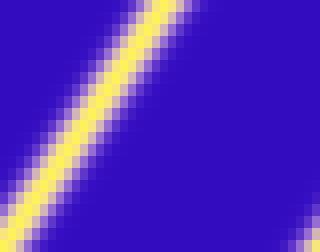
\includegraphics[width=0.48\textwidth]{../figures/q2_true_motion.png}
\hfill
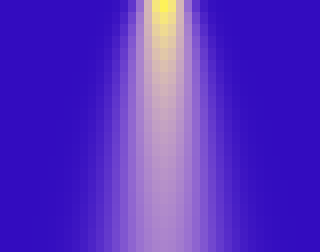
\includegraphics[width=0.48\textwidth]{../figures/q2_undirected_layer.png}
\caption{Left: true backward shift. Right: undirected layer ($a=0$, $b=1/2$).}
\end{figure}

\subsection*{(b) Directed weights}
Exact next snapshot for backward motion: $a=0$, $w_{-}=0$, $w_{+}=1$, i.e.\ $\hat x_i(t+1)=x_{i+1}(t)$.
As a 1D convolution, the kernel on $[x_{i-1},x_i,x_{i+1}]$ is $[0,0,1]$. On the ring, use circular padding / wrap-around.

Knowing which neighbour is ahead removes the symmetry that forced $w_{-}=w_{+}$ in (a).

\subsection*{(c) Equal neighbour weights + history}
\textbf{(i)} Under backward motion, $x_i(t-1)=x_{i-1}(t)$. Choose $a=0$, $b=1$, $c=-1$:
\[
\hat x_i(t+1)=x_{i-1}(t)+x_{i+1}(t)-x_i(t-1)=x_{i+1}(t).
\]
\textbf{(ii)} Under forward motion, $x_i(t-1)=x_{i+1}(t)$. The same coefficients give
\[
\hat x_i(t+1)=x_{i-1}(t)+x_{i+1}(t)-x_{i+1}(t)=x_{i-1}(t),
\]
so they still work.
\textbf{(iii)} History tells which neighbour matches the past reading, so the cancelation picks the correct direction even though the two spatial weights stay equal.

\section*{Question 3 --- Dataset preparation}

\subsection*{Q3(a)}
Source: LargeST CA files (HuggingFace processed release), San Diego = PeMS district 11 ($N=716$). Years 2020--2021. Original sampling is 5 minutes; we resample with a 15-minute \textbf{mean} (treat values as average flow rates, not vehicle counts). Missing values: time-wise linear interpolate per sensor, then fill leftovers with 0. Missing fraction before fill is reported in \texttt{results/q3\_summary.json}.

\begin{figure}[H]
\centering
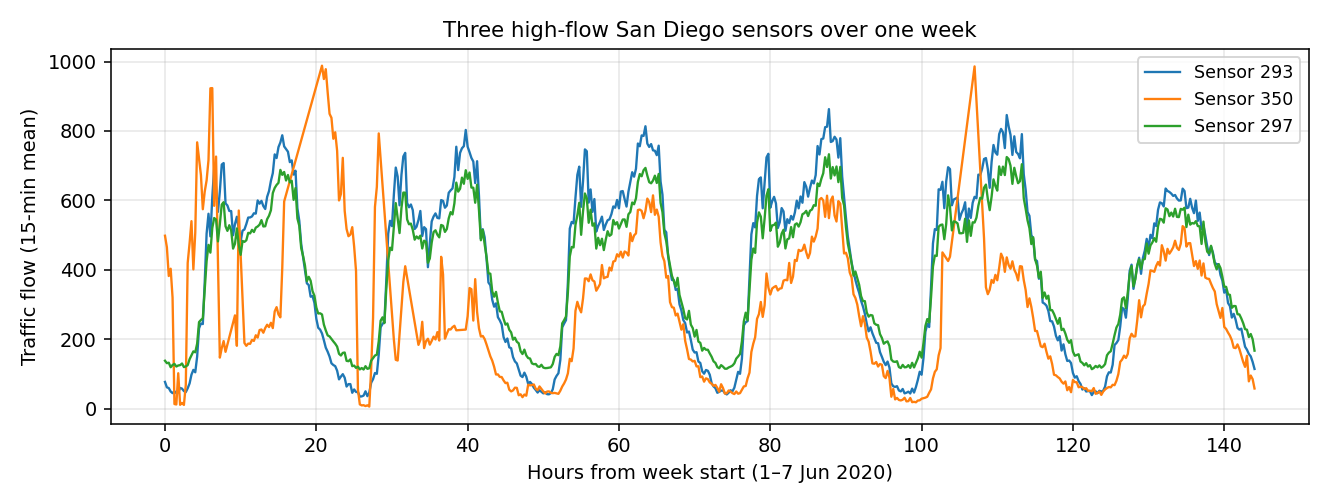
\includegraphics[width=0.85\textwidth]{../figures/q3_three_sensors_week.png}
\caption{Three high-flow SD sensors over one week (15-min series).}
\end{figure}

\subsection*{Q3(b)}
Adjacency is the LargeST road-distance matrix restricted to SD sensors (same order as the flow tensor). Nonzero $A_{ij}$ means sensors $i$ and $j$ are linked by a (thresholded) road-network distance weight. Node/edge counts, symmetry check, heatmap and degree histogram are in the figures/results folder.

\begin{figure}[H]
\centering
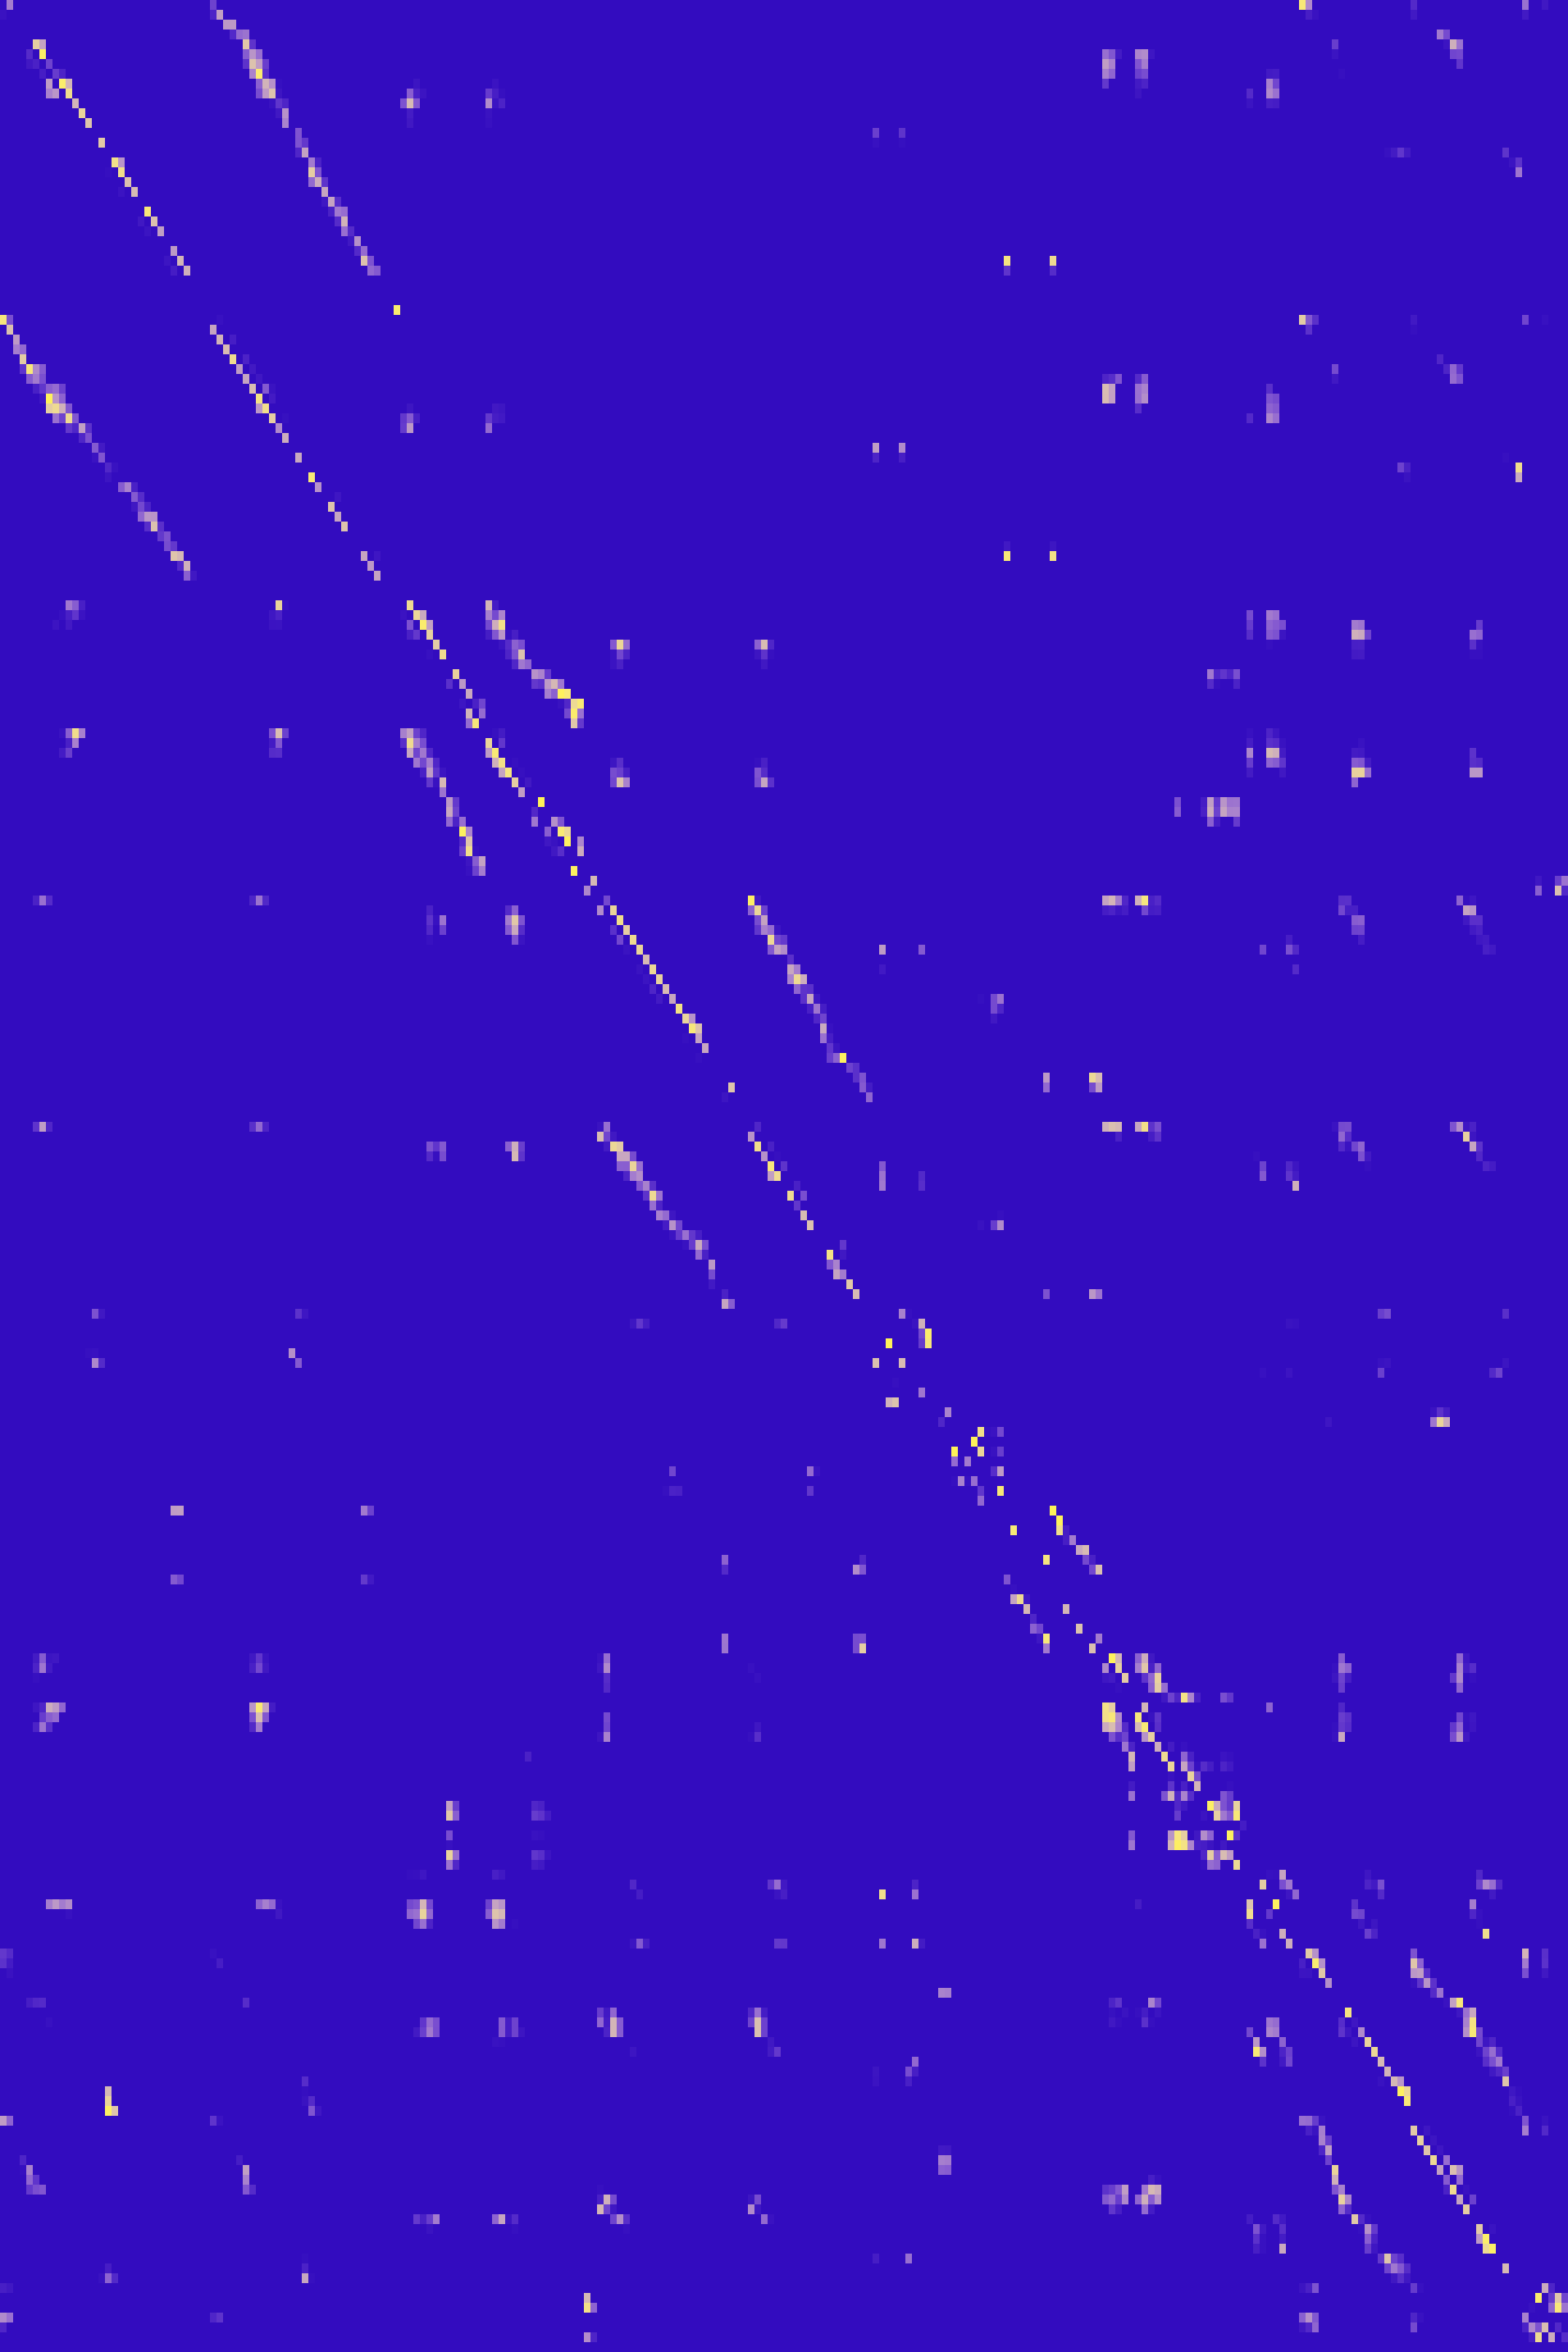
\includegraphics[width=0.45\textwidth]{../figures/q3_adj_heatmap.png}
\hfill
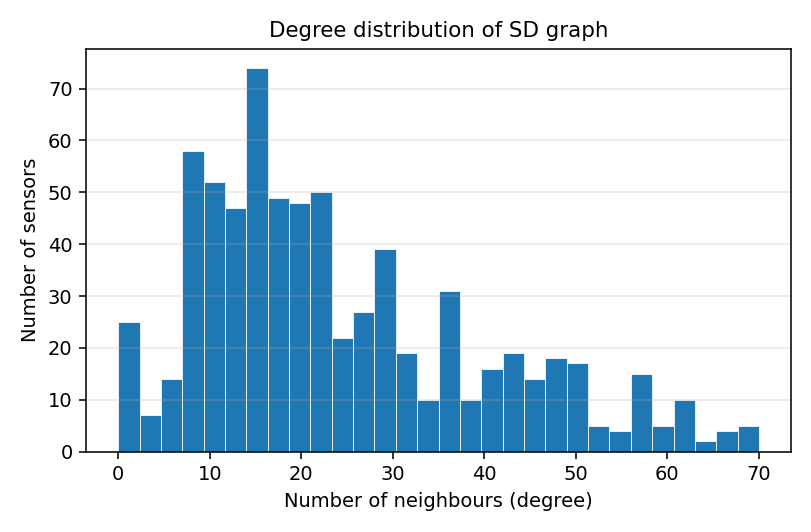
\includegraphics[width=0.45\textwidth]{../figures/q3_degree_hist.png}
\caption{SD adjacency heatmap (downsampled) and degree histogram.}
\end{figure}

\subsection*{Q3(c)}
For a high-degree sensor $v$, one-hop neighbours are direct road links; two-hop neighbours are sensors reachable in two edges. Neighbours help because congestion spreads along connected roads. One-hop aggregates immediate neighbours; two-hop reaches farther structure. Too many GCN layers can over-smooth node features so sensors look alike and forecasting gets worse.

\section*{Question 4 --- Spatio-temporal forecasting}

\subsection*{Q4(a)}
Windows: 8 past steps $\to$ 4 future steps (1 hour). Splits: train 2020; val Jan--Mar 2021; test Apr--Dec 2021. Windows do not cross split borders. Mean/std from training only.

\subsection*{Q4(b)--(c)}
Model: temporal Conv1d encoder per sensor $\to$ optional graph convolution $H=\mathrm{ReLU}(\hat A Z W)$ $\to$ MLP head for 4 leads. Loss: MAE on normalised flow. Metrics reported in original units. Temporal-only baseline drops the graph block. See Table in Q6.

\section*{Question 5 --- Fixed / adaptive / hybrid adjacency}

\subsection*{Q5(a)} Fixed: $\hat A=D^{-1/2}(A+I)D^{-1/2}$ (matrix is nearly symmetric).
\subsection*{Q5(b)} Adaptive: $A_{\mathrm{ad}}=\mathrm{Softmax}(\mathrm{ReLU}(E_1 E_2^\top))$ with top-$k{=}15$ before softmax. Gradients flow through selected logits.
\subsection*{Q5(c)} Hybrid: $A_{\mathrm{hy}}=\alpha\hat A+(1-\alpha)A_{\mathrm{ad}}$ with learnable $\alpha\in(0,1)$ after sigmoid.

\begin{figure}[H]
\centering

\includegraphics[width=0.55\textwidth]{../figures/q5_learned_adj.png}
\caption{Learned adaptive adjacency (downsampled heatmap).}
\end{figure}

\section*{Question 6 --- Results}

\subsection*{Q6(a)}
\begin{table}[H]
\centering
\rowcolors{2}{white}{gray!8}
\begin{tabular}{llrrr}
\rowcolor{tablehead}
\textbf{Model} & \textbf{Adjacency} & \textbf{MAE} & \textbf{RMSE} & \textbf{Train time (s)}\\
\midrule
Temporal-only & None & --- & --- & ---\\
STGNN & Fixed & --- & --- & ---\\
STGNN & Adaptive & --- & --- & ---\\
STGNN & Hybrid & --- & --- & ---\\
\end{tabular}
\end{table}
\noindent\textit{Numbers filled automatically from \texttt{results/comparison\_table.json} after training.}

\begin{figure}[H]
\centering
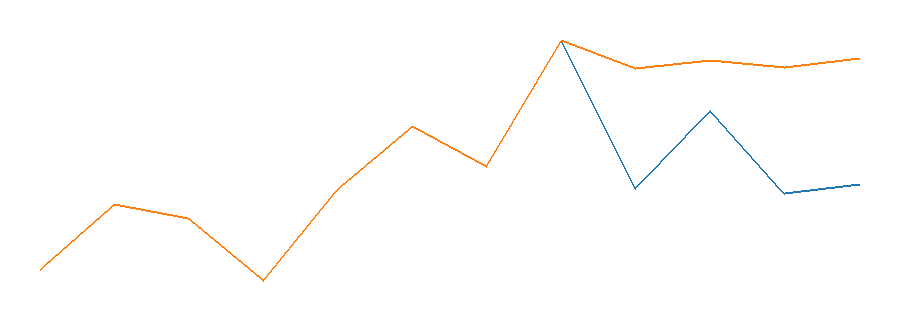
\includegraphics[width=0.32\textwidth]{../figures/q6_sensor_A_pred.png}
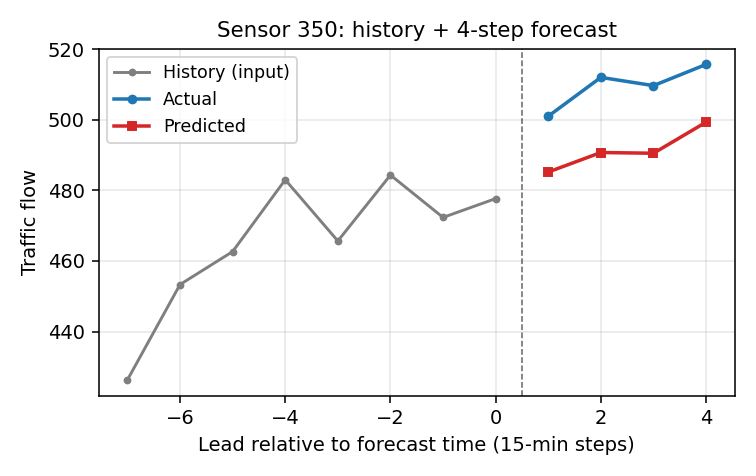
\includegraphics[width=0.32\textwidth]{../figures/q6_sensor_B_pred.png}
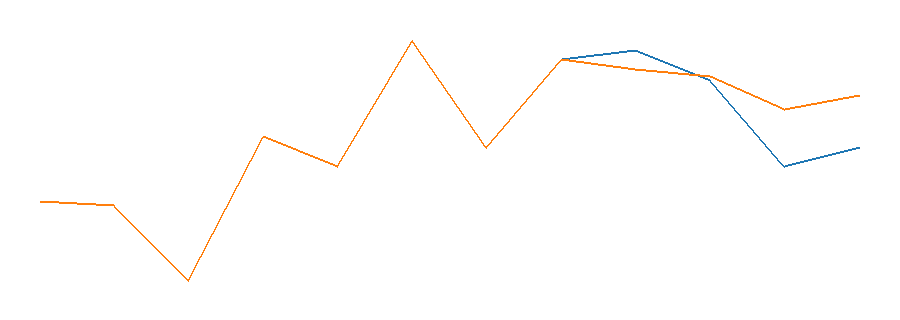
\includegraphics[width=0.32\textwidth]{../figures/q6_sensor_C_pred.png}
\caption{Predicted vs actual (history + 4-step horizon) for three sensors.}
\end{figure}

\subsection*{Q6(b)}
We compare the strongest learned edges with the road graph (overlap fraction in \texttt{graph\_analysis.json}). Learned links can connect sensors that are not road-adjacent when they share similar traffic patterns. Adaptive graphs help when physical distance misses functional dependence; they can hurt if the learned matrix is noisy or overfits.

\subsection*{Q6(c)}
Lower error does not prove the learned graph equals real roads --- it only means the matrix is useful for prediction. Hybrid can win by keeping reliable road edges while adding data-driven shortcuts. A static graph ignores time-of-day changes (rush hour vs night), so a future model could use time-varying or multi-graph structure.

\section*{Question 7 --- Reproducibility}
\begin{itemize}[leftmargin=*]
\item Code: repository linked on page 1. Run order in \texttt{README.md}.
\item Seed 42; hidden 24; epochs 12; batch 32; lr $10^{-3}$; input 8; horizon 4; adaptive top-$k=15$.
\item Hardware and measured times: see \texttt{results/train\_details.json}.
\item AI use note: Cursor agent used for coding/debugging; prompts and edits summarised in the appendix below.
\end{itemize}

\section*{Appendix --- AI tool note}
Prompt (summary): complete DL4STG PA3 from the PDF, unique write-up, simple report with tables/plots.\\
Edits: checked maths by hand for Q1--Q2; kept the STGNN small for CPU; filled metrics from local runs only.

\end{document}
